\documentclass[Main.tex]{subfiles} 
\begin{document}

\subsection{Gr�nseflader til eksternt software}
Her beskrives gr�nsefladerne for de software delsystemer, der er blevet udviklet som et separat projekt.\\
Der er blevet udviklet en simulator sidel�bende med projektet, da det blev n�dvendigt at have mulighed for at simulere en bus der k�re p� en rute, da der ikke var mulighed for at f� positions data for en rigtig bus. Et andet form�l med simulatoren er at g�re det muligt at teste forskellige situationer der kan forekomme i systemet. 
\subsubsection{Simulator}
N�r simulatoren bliver startet vil gr�nsefladen se ud, som vist p� figur \ref{fig:SimulatorViewStart}. Herfra kan der ved 'BusNr:' v�lges hvilken busrute, busserne skal k�re p�. Update speed bestemmer hvor ofte positionen for busserne skal opdateres, her er '1' standardv�rdien for systemet. I simulation mode, v�lges der hvilken form for simulation der skal startes, dette kan v�re: 'Use single bus on route', 'Use all busses on chosen route' og 'Use all busses in system'.
'Use single bus on route' vil simulere en enkel bus der k�re p� den valgte rute, hvor 'Use all busses on chosen route' vil simulere alle de busser der er knyttet til den valgte rute. Ved valg af 'Use all busses in system' vil alle busser i hele systemet blive simuleret p� deres tilknyttet rute, og det er derfor ligemeget hvilken busrute der blev valgt i starten. Under 'Bus Direction' kan der v�lges om busserne skal k�re i en bestemt retning, eller om de alle skal k�re i tilf�ldige retning. sidst kan der v�lges hvor hurtig busserne skal k�re, her der er mulighed for at s�tte hastigheden mellem 30 og 1000 km/t. Simulatoren kan nu startes p� to forskellige m�der, enten hvor busserne alle starter tilf�ldige steder p� deres rute, eller om alle busserne skal starte fra rutens startpunkt.
\begin{figure}[H]
	\centering
	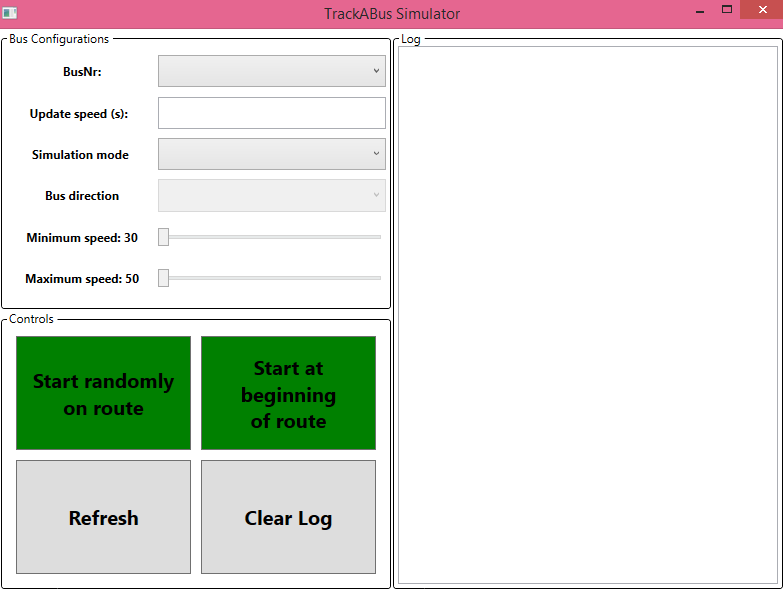
\includegraphics[scale=0.5]{./Diagrammer/Billeder/SimulatorViewStart.png}
	\caption{Gr�nseflade for simulator}
	\label{fig:SimulatorViewStart}
\end{figure}
\noindent
P� figur \ref{fig:SimulatorViewStarted} kan ses hvordan det kan se ud efter en simulation er startet. Her kan det ses et log vindue i h�jre side, der kommer med opdateringer om busserne, og eventuelle fejlbeskeder. De to sidste knapper p� simulatoren, 'Refresh' og 'clear log' bruges henholdsvis til at hente de nyeste ruter og busser fra databasen, og til at slette alt hvad der st�r i log vinduet.
\begin{figure}[H]
	\centering
	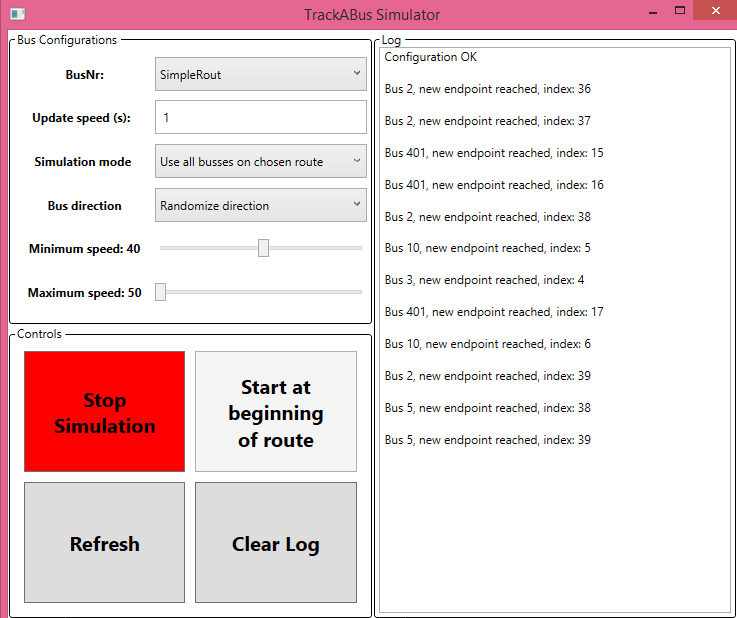
\includegraphics[scale=0.5]{./Diagrammer/Billeder/SimulatorViewStarted.png}
	\caption{Gr�nseflade for simulator efter den er blevet configureret og startet}
	\label{fig:SimulatorViewStarted}
\end{figure}
\noindent

\end{document}